\section{Introduction}
\label{sec:intro}
With the emergence of reasoning-oriented models such as DeepSeek-R1~\citep{DeepSeek-R1}, Reinforcement Learning (RL) has become an increasingly important paradigm for post-training large language models (LLMs), particularly for improving instruction following, alignment, and reasoning capabilities~\citep{Yu2025DAPO,Open-Reasoner-Zero,qwen3technicalreport}. 
Due to the massive scale of LLM, modern LLM RL pipelines often separate rollout generation from gradient computation: responses are sampled by an inference engine (e.g. vLLM~\citep{vllm} or SGLang~\citep{zheng2024sglang}), whereas log-probabilities and updates are computed by a training engine (e.g. FSDP~\citep{fsdp} or Megatron~\citep{megatron}). 
Even under synchronized parameters, implementation differences in precision, decoding, or serving backends can make the training policy $\textcolor{blue}{\pi}$ and inference policy $\textcolor{red}{\mu}$ assign different probabilities to the same trajectories.
This inevitably creates the notorious \textit{training-inference mismatch} issue~\citep{mismatch1,mismatch2}. 

Existing algorithmic and infrastructure remedies reduce this mismatch by correcting sampler-side ratios~\citep{mismatch1}, filtering unstable samples~\citep{mismatch2}, decaying learning rates~\citep{lrdecay}, or narrowing system-level discrepancies~\citep{li2026qurl,fp16}. 
These works aim to address the mismatch on the training side by improving the stability of the policy optimization process.
However, due to the ever-existing training-inference mismatch, there is no guarantee that effective improvement of the training policy necessarily take the same effect for the inference policy.



\begin{figure}
    \centering
    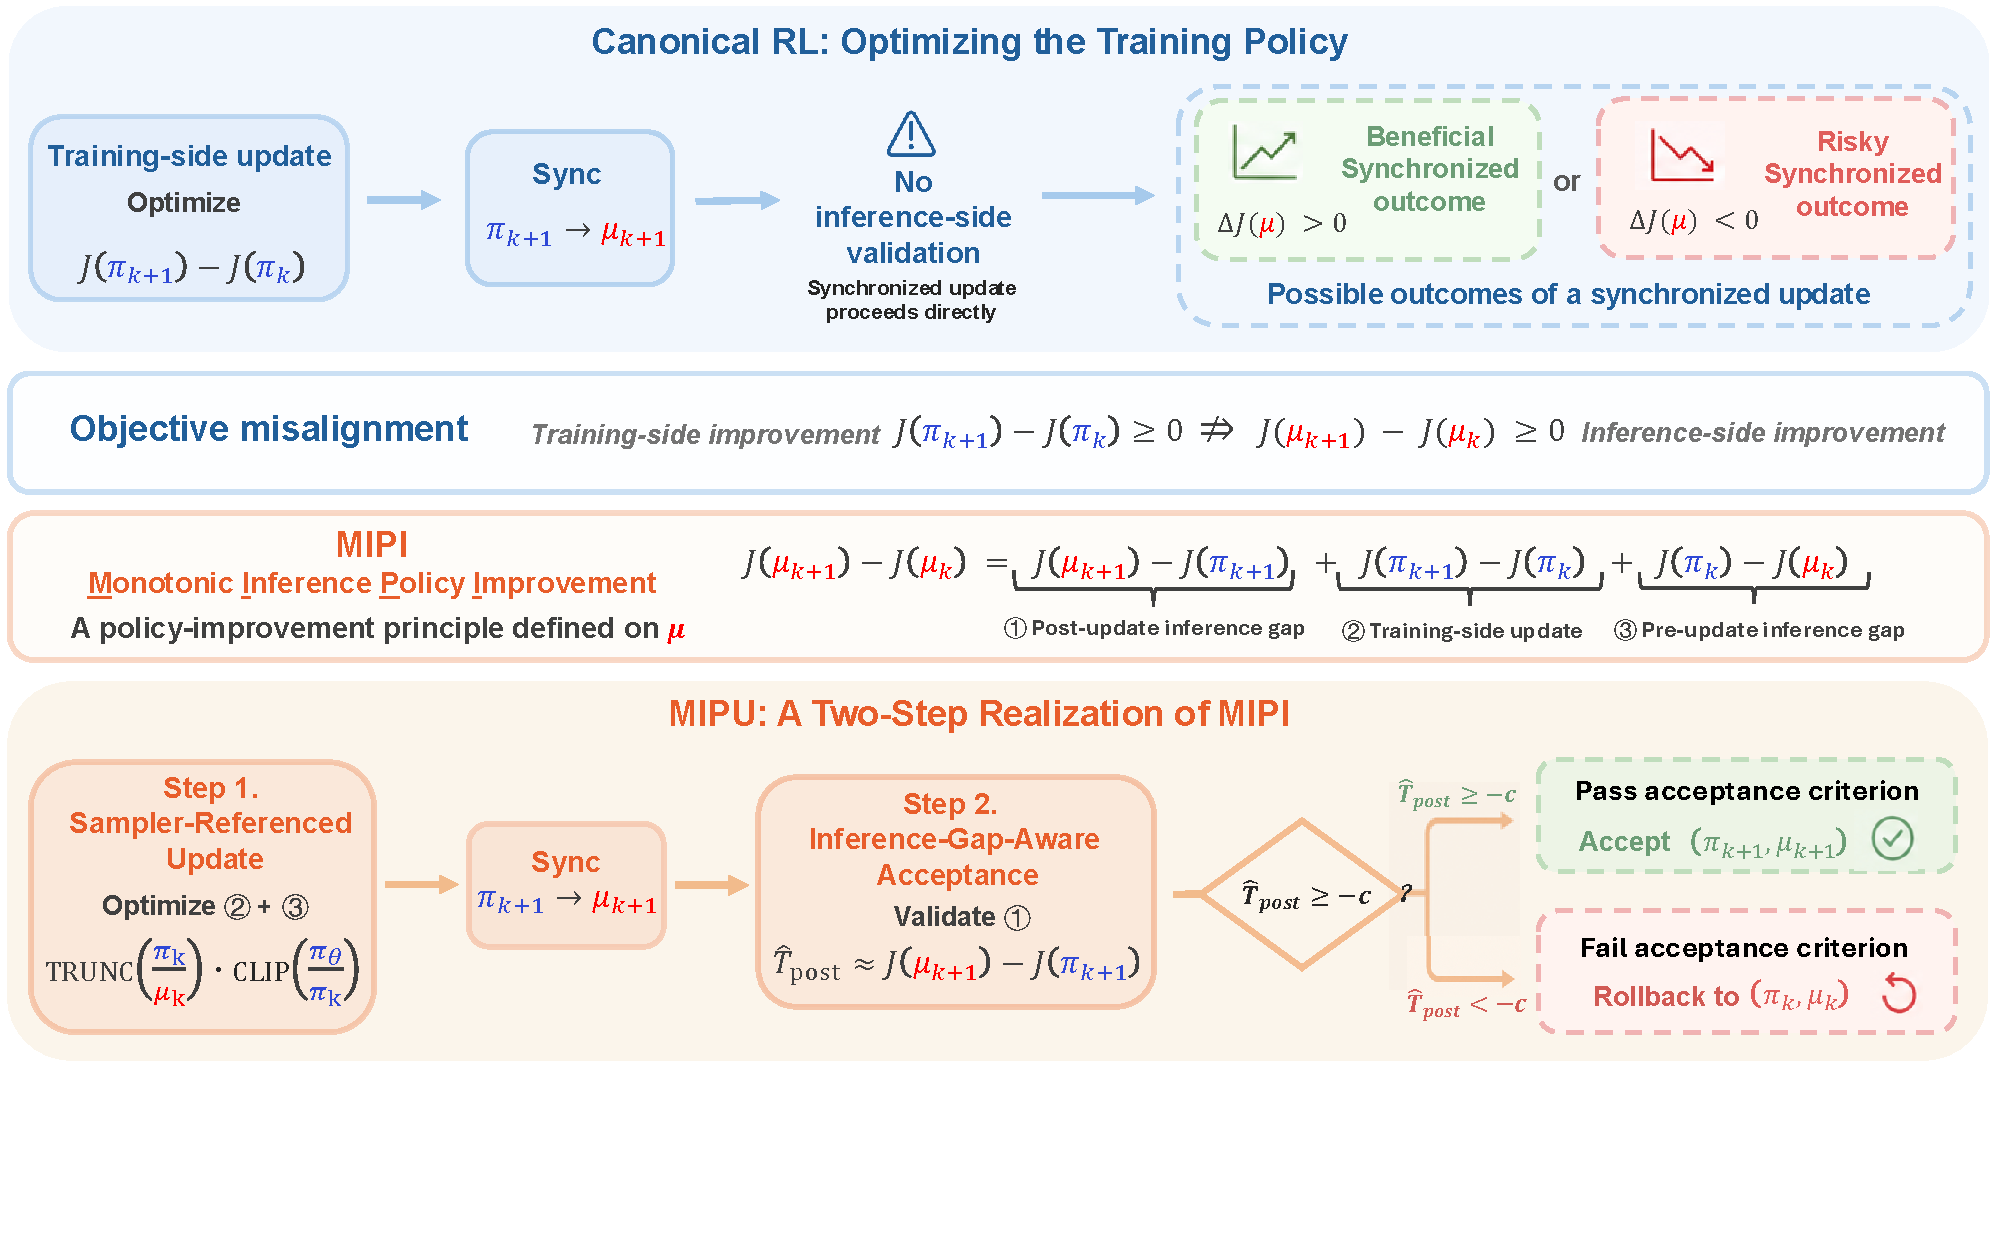
\includegraphics[width=1\linewidth]{fig/main_0615v1.pdf}
    \caption{\textbf{Monotonic Inference Policy Update (MIPU) resolves the \textit{Objective Misalignment} issue of LLM RL. }
Canonical LLM RL accepts synchronized updates by a training-side objective, which does not necessarily imply improvement of the inference policy.
Here, $\textcolor{blue}{\pi}$ and $\textcolor{red}{\mu}$ denote the training policy and inference policy respectively, $c$ is a tolerance parameter accounting for proxy noise.
To address this mismatch, we propose a new principle as monotonic improvement on the inference-policy trajectory (the \textbf{MIPI} principle).
\textbf{MIPU} realizes this principle with two steps: \textbf{Step 1 optimizes Terms \textcircled{2}+\textcircled{3}, while Step 2 estimates and validates Term \textcircled{1}, jointly covering all three terms in the MIPI decomposition.}
}
\vspace{-0.5cm}
    \label{fig:method}
\end{figure}

This suggests an \textit{objective-level} view of training-inference mismatch.
Since the policy used for rollout and deployment is induced by the inference engine, a model update should not be judged solely by whether it improves the training policy, i.e., the canonical optimization objective of LLM RL algorithms.
Instead, the more natural question is:
\vspace{-0.1cm}
\begin{center}
\textit{Whether synchronizing this update actually produces a better inference policy ?}
\end{center}
\vspace{-0.1cm}
In face of the objective misalignment revealed above, in this work we aim to break the canonicity of improving the training policy, and propose a new policy optimization principle for LLM RL, named \textbf{\underline{M}onotonic \underline{I}nference \underline{P}olicy \underline{I}mprovement ({MIPI})}: the policy optimization objective should be established to improve the performance of the inference policy monotonically.
Following this principle, we propose a two-step LLM RL framework, called \textbf{\underline{M}onotonic \underline{I}nference \underline{P}olicy \underline{U}pdate (MIPU)}.
As illustrated in~\autoref{fig:method}, the recipe of \textbf{MIPU} is to decompose the \textbf{MIPI} objective (i.e., $J(\textcolor{blue}{\mu_{k+1}})-J(\textcolor{blue}{\mu_k})$) into three terms, and optimize it via a sampler-referenced policy
update step (i.e., the direct `Step 1') and a inference-gap-aware acceptance step (i.e., the indirect `Step 2').
For Step 1, the training engine performs a sampler-referenced policy update to generate a candidate model that theoretically ensures the halfway monotonicity $J(\textcolor{red}{\pi_{k+1}})-J(\textcolor{blue}{\mu_k}) \ge 0$.
For Step 2, the synchronized candidate is evaluated through an inference-gap-aware acceptance criterion, where the accepted update further ensures the remaining half monotonicity $J(\textcolor{blue}{\mu_{k+1}}) -J(\textcolor{red}{\pi_{k+1}}) \ge 0$.

In the experiments, we evaluate \textbf{MIPU} under FP8-quantized rollout, a high-mismatch setting where inference-side quantization amplifies the training-inference discrepancy. 
Across Qwen3-4B and Qwen3-1.7B, \textbf{MIPU} achieves the best average performance and more stable training dynamics. 
Further analysis shows that Step~1 improves candidate updates, while Step~2 filters unreliable synchronized candidates using an inference-side criterion.

The contributions of this paper are summarized as follows:
\begin{itemize}
    \item We propose a new learning objective for LLM RL, i.e., \textbf{MIPI}, which aligns with the purpose de facto and circumvents the training-inference mismatch issue.
    \item We propose a new LLM RL framework, i.e., \textbf{MIPU}, that realizes the \textbf{MIPI} principle in a two-step manner. \textbf{MIPU} allows flexible implementation of both sampler-referenced policy update step and inference-gap-aware update acceptance step.
    \item Experiments under FP8-quantized rollout show that \textbf{MIPU} improves both performance and training stability. And additional analysis verifies the complementary roles of Step~1 and Step~2 in candidate construction and inference-gap-aware acceptance.
\end{itemize}
